\chapter*{Introduction: The Triangle That Swallowed the Universe}
\addcontentsline{toc}{chapter}{Introduction: The Triangle That Swallowed the Universe}
\markboth{Introduction}{Introduction}



\section{The Puzzle on the Bathroom Tiles}


Suppose, one rainy Saturday afternoon, you find yourself staring at the bathroom floor. The tiles are square --- plain white, one inch on a side --- and as you wait for the bathtub to fill, your mind begins to wander. You start counting. Nine tiles would cover a $3 \times 3$ square. Sixteen tiles would cover a $4 \times 4$ square. Twenty-five tiles would cover a $5 \times 5$ square. And then, unbidden, a small miracle appears:

\[
9 + 16 = 25.
\]

You blink. Three squared plus four squared equals five squared. You check it again:

\[
3^2 + 4^2 = 9 + 16 = 25 = 5^2.
\]

If you were to cut out a $3 \times 3$ square of tiles and a $4 \times 4$ square of tiles, you could rearrange all twenty-five tiles into a perfect $5 \times 5$ square --- no tiles left over, no gaps, no overlaps. The two smaller squares, pooling their resources, have exactly enough material to build the larger one.

Is this a coincidence? A one-off numerical curiosity, like the fact that $12 + 3 = 15$ or that Tuesday comes after Monday? Or is it a specimen of something --- a single butterfly pinned in a case that contains thousands more?

Here is a game to find out. Try to discover other triples of whole numbers $(a, b, c)$ for which

\[
a^2 + b^2 = c^2.
\]

Take a few minutes before reading on. Use scratch paper. You will almost certainly find $(3, 4, 5)$ first --- we already have that one. After some effort you might stumble on $(5, 12, 13)$: check it and see, $25 + 144 = 169$, and $13^2 = 169$. Splendid. What about $(8, 15, 17)$? We compute $64 + 225 = 289 = 17^2$. Yes! And $(7, 24, 25)$: $49 + 576 = 625 = 25^2$. They keep coming.

\begin{figure}[htbp]
\centering
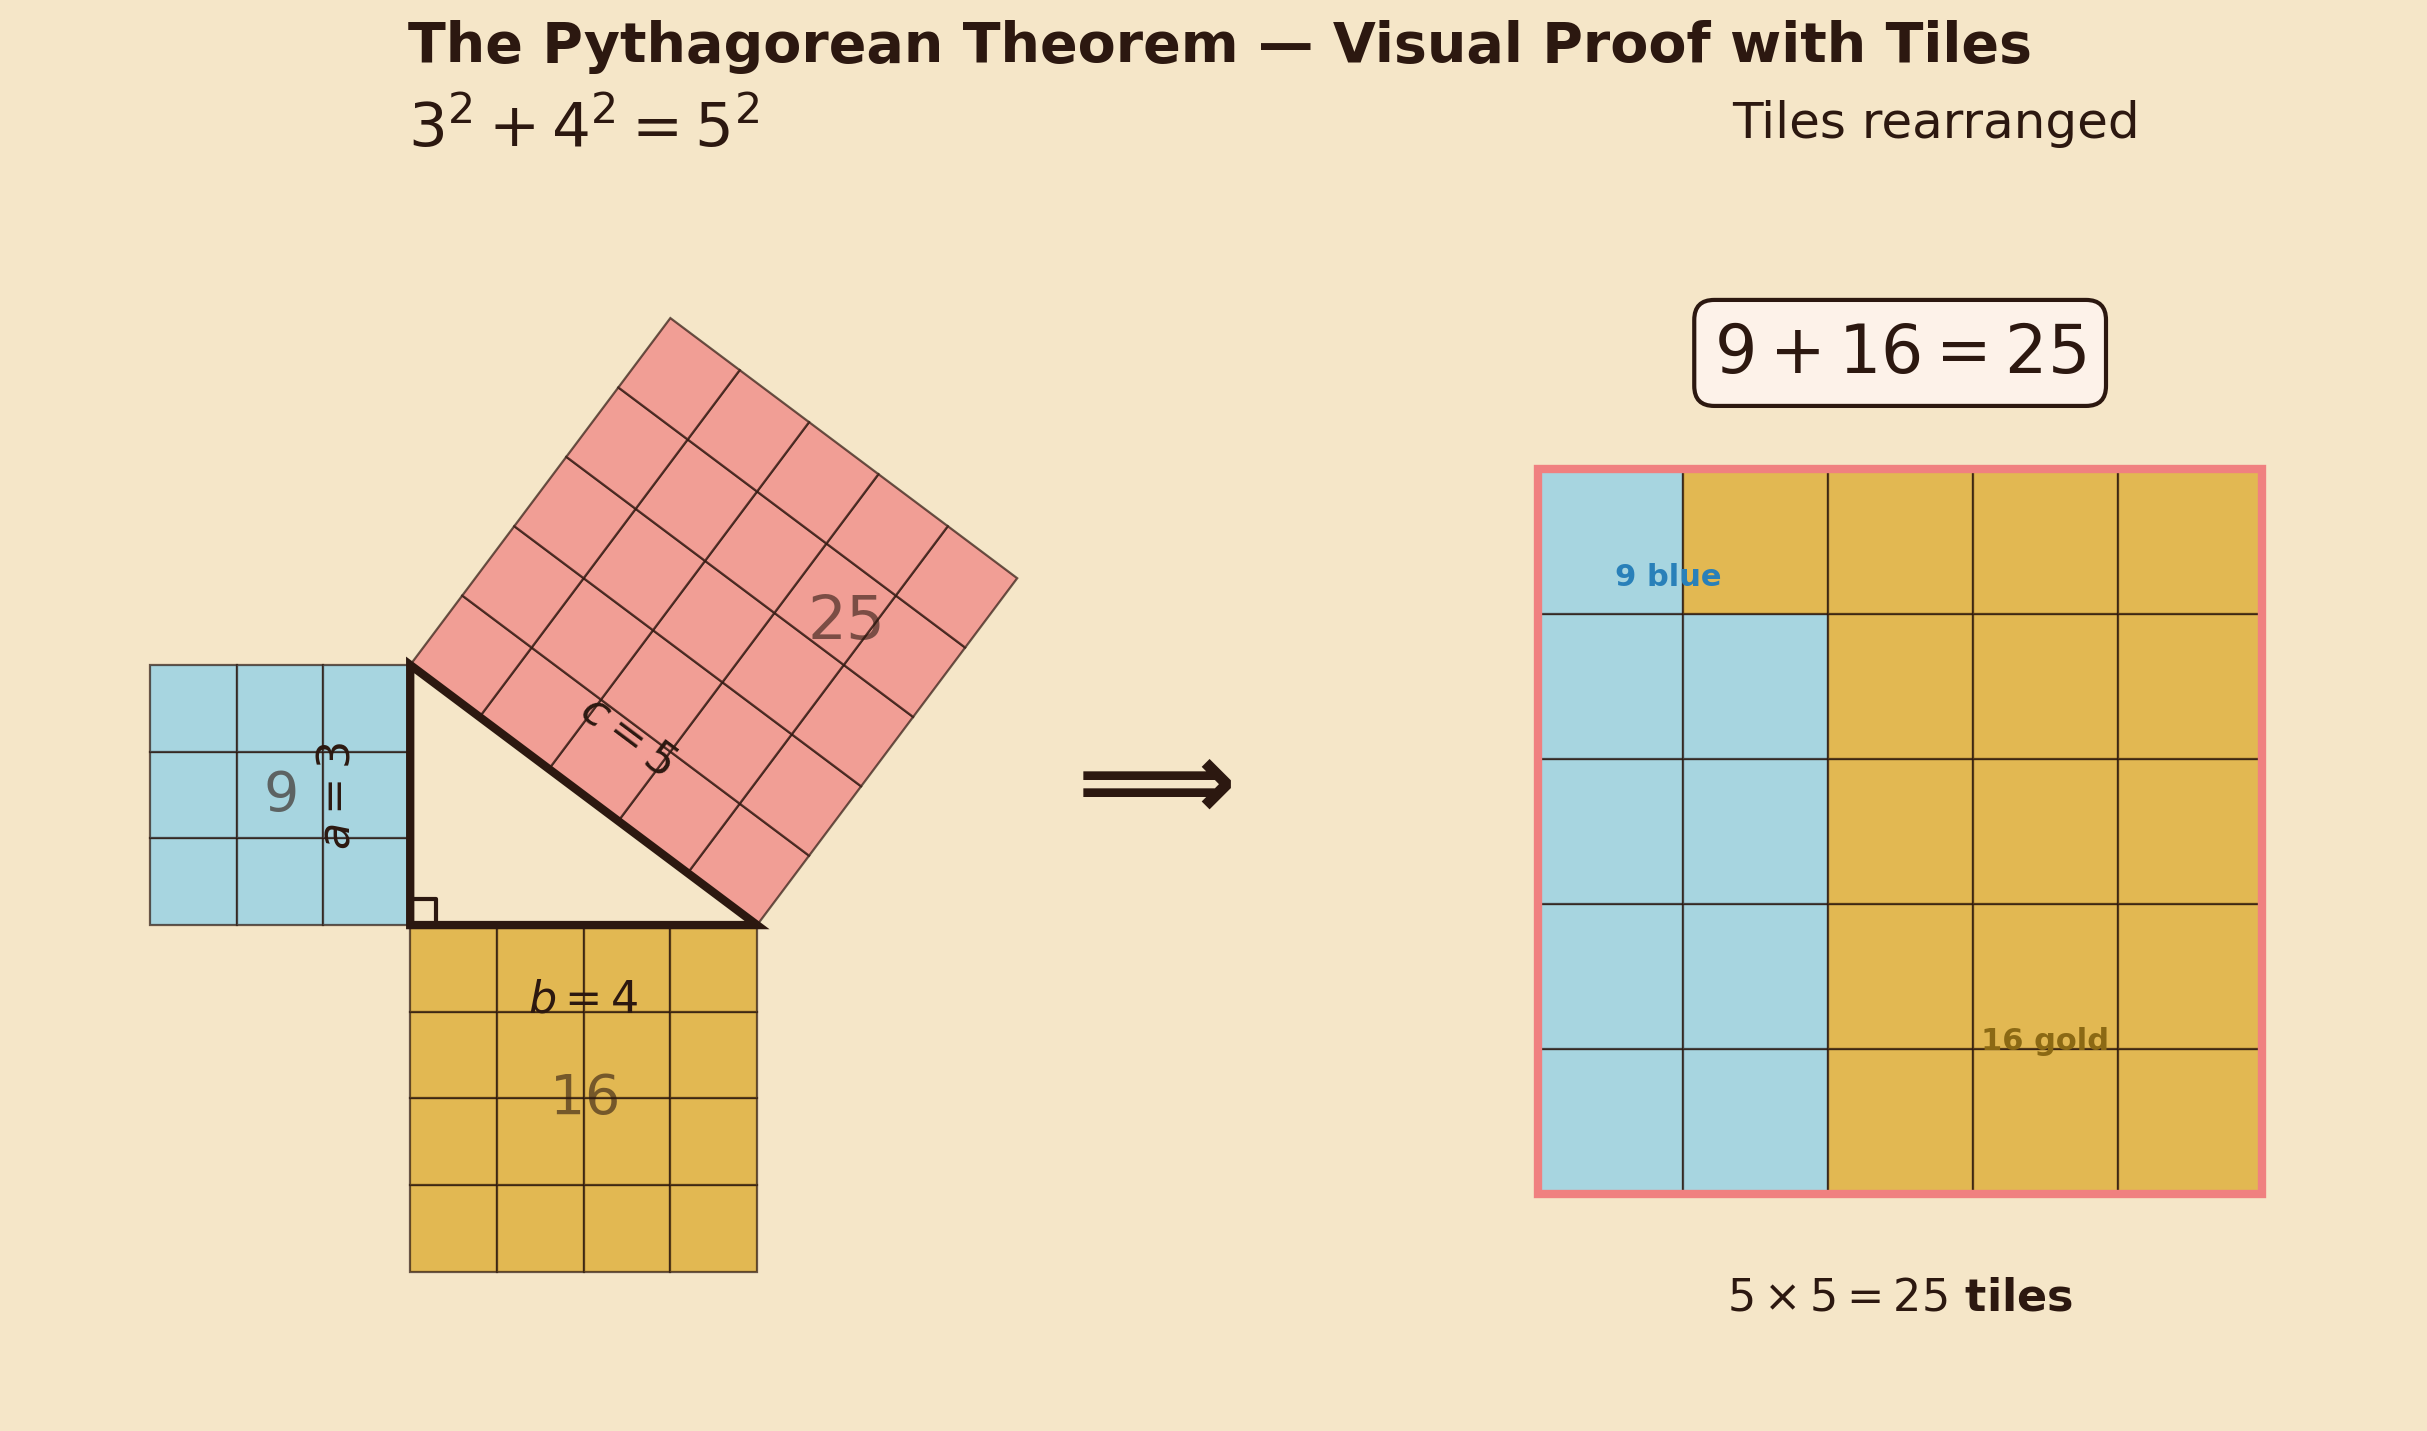
\includegraphics[width=0.82\textwidth,keepaspectratio]{images/introduction_fig01_pythagorean_squares.png}
\caption{A large, beautifully rendered depiction of a right triangle with legs labeled $a = 3$ and $b = 4$ and hypotenuse $c = 5$.}
\end{figure}


Now here is the puzzle that will occupy us for the rest of this book --- and, if you let it, for the rest of your mathematical life:

\begin{quote}
\textbf{Can you ever run out?} Is there a largest Pythagorean triple\index{Pythagorean triple}, after which no new ones exist? Or do they go on forever? And if they go on forever --- is there a \textit{pattern}? A system? A map?
\end{quote}


\ornbreak



\subsection{A Four-Thousand-Year-Old Secret}


Before we answer, let us pause to appreciate how old this question is. In 1945, the historians Otto Neugebauer\index{Neugebauer, Otto} and Abraham Sachs published a translation of a small clay tablet, roughly the size of a modern smartphone, that had been sitting in the Columbia University collection since the 1920s. The tablet, catalogued as \textit{Plimpton 322\index{Plimpton 322}}, had been baked in Mesopotamia around 1800 BCE --- more than a thousand years before Pythagoras was born.

What Neugebauer and Sachs found on it was astonishing: a table of fifteen rows and four columns, each row containing numbers that, when properly interpreted, form a Pythagorean triple. Row 1 gives the triple $(119, 120, 169)$. Check: $119^2 + 120^2 = 14{,}161 + 14{,}400 = 28{,}561 = 169^2$. Row 4 gives $(12{,}709,\; 13{,}500,\; 18{,}541)$. These are not small numbers. These are not lucky guesses. Whoever inscribed this tablet had a \textit{method} --- a systematic procedure for generating triples of any size.

What was that method? We cannot be sure, but the leading hypothesis is breathtaking in its simplicity. It appears that the Babylonian scribe knew, in some form, the following recipe: choose two whole numbers $m$ and $n$, with $m > n > 0$, and compute

\[
a = m^2 - n^2, \qquad b = 2mn, \qquad c = m^2 + n^2.
\]

Then $a$, $b$, and $c$ will always satisfy $a^2 + b^2 = c^2$.

This is not a guess --- it is a provable fact, and the proof is one line of algebra that a patient high-school student can verify:

\[
a^2 + b^2 = (m^2 - n^2)^2 + (2mn)^2 = m^4 - 2m^2 n^2 + n^4 + 4m^2 n^2 = m^4 + 2m^2 n^2 + n^4 = (m^2 + n^2)^2 = c^2.
\]

The middle terms $-2m^2 n^2$ and $+4m^2 n^2$ obligingly combine to $+2m^2 n^2$, and the whole expression collapses into a perfect square. It is one of those algebraic coincidences that feels too clean to be an accident --- and indeed, it is no accident at all. It is the shadow of a deep geometric truth that we will spend the rest of this introduction illuminating.

Let us test-drive the formula. Setting $m = 2$ and $n = 1$:

\[
a = 4 - 1 = 3, \qquad b = 2 \cdot 2 \cdot 1 = 4, \qquad c = 4 + 1 = 5.
\]

Our old friend $(3, 4, 5)$. Now $m = 3$, $n = 2$:

\[
a = 9 - 4 = 5, \qquad b = 12, \qquad c = 9 + 4 = 13.
\]

The triple $(5, 12, 13)$ --- precisely the one we found by trial and error. And $m = 4$, $n = 1$:

\[
a = 16 - 1 = 15, \qquad b = 8, \qquad c = 17.
\]

So $(15, 8, 17)$ --- or equivalently $(8, 15, 17)$, since we don't mind which leg is which.

\begin{figure}[htbp]
\centering
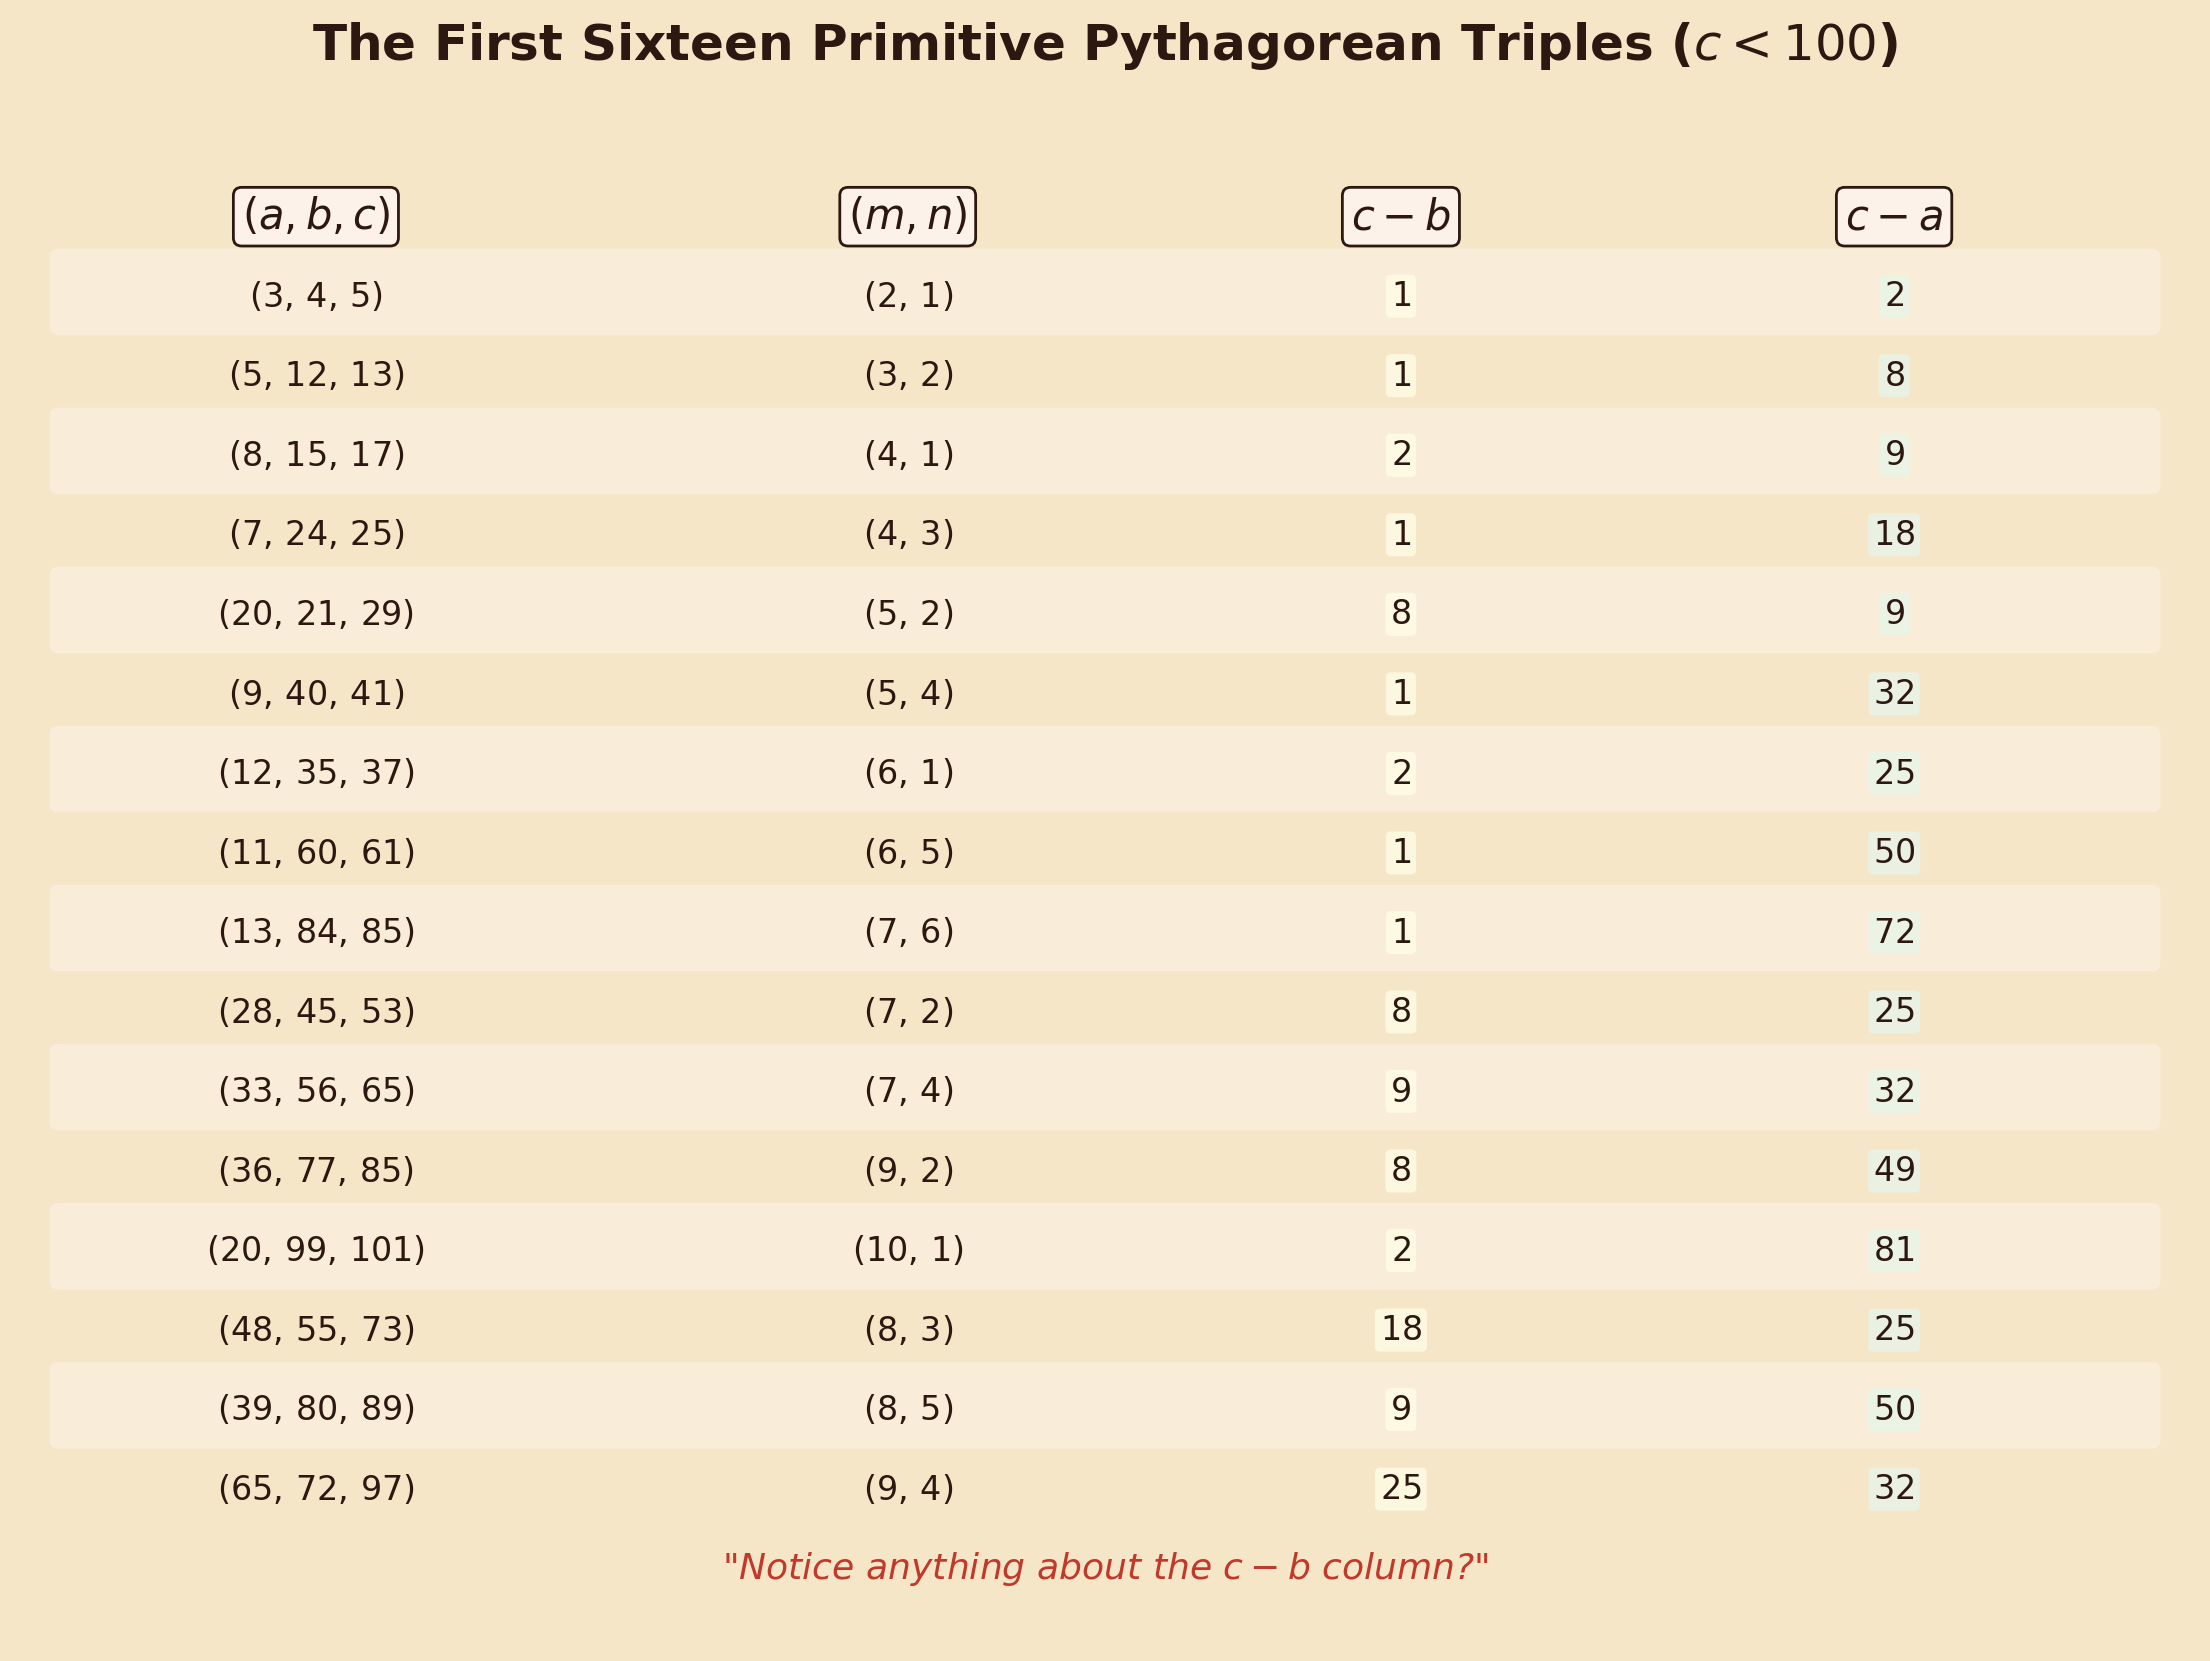
\includegraphics[width=0.82\textwidth,keepaspectratio]{images/introduction_fig02_primitive_triples_table.png}
\caption{A table of the first sixteen primitive Pythagorean triples, organized in four columns.}
\end{figure}


Since we can choose $m$ and $n$ to be as large as we please, the formula generates infinitely many triples. The bathroom tiles never run out. But a new question immediately surfaces: does this formula generate \textit{all} Pythagorean triples, or only some of them? And among the triples it generates, are there repetitions --- different choices of $(m, n)$ that happen to produce the same triple?

The answer to both questions is surprisingly subtle, and it hinges on a distinction that will matter enormously in everything that follows.


\ornbreak



\subsection{Primitive vs. Imprimitive: The Genealogy of Triples}


Call a Pythagorean triple \textit{primitive} if the three numbers $a$, $b$, and $c$ share no common factor greater than $1$. The triple $(3, 4, 5)$ is primitive: no integer except $1$ divides all three. But the triple $(6, 8, 10)$ is \textit{not} primitive --- it is simply $(3, 4, 5)$ multiplied through by $2$. The triple $(9, 12, 15)$ is $(3, 4, 5)$ multiplied by $3$. In fact, every Pythagorean triple is either primitive or a positive integer multiple of a primitive one. (If $d$ divides $a$, $b$, and $c$, then $a/d$, $b/d$, $c/d$ is still Pythagorean --- just divide the equation $a^2 + b^2 = c^2$ through by $d^2$.)

This means that to understand \textit{all} Pythagorean triples\index{Pythagorean triple}, it suffices to understand the \textit{primitive} ones. Everything else is just rescaling. And here is the beautiful theorem, attributed to Euclid\index{Euclid} but refined over the centuries:

\begin{quote}
\textbf{Euclid's Classification.} Every primitive Pythagorean triple $(a, b, c)$ with $a$ odd and $b$ even is given by
$$a = m^2 - n^2, \qquad b = 2mn, \qquad c = m^2 + n^2$$
where $m > n > 0$, $\gcd(m, n) = 1$, and $m - n$ is odd. Moreover, different valid pairs $(m, n)$ always produce different triples.
\end{quote}

The two extra conditions --- that $m$ and $n$ be coprime (sharing no common factor) and of opposite parity (one even, one odd) --- are precisely what prevents repetitions and ensures primitivity. Without them, you get imprimitive triples sneaking in: for example, $m = 2$, $n = 2$ gives $(0, 8, 8)$, which is degenerate, and $m = 3$, $n = 1$ gives $(8, 6, 10) = 2 \times (4, 3, 5)$, which is imprimitive.

With these conditions in place, the Euclid parametrization is a \textit{perfect census}. Every primitive triple\index{primitive triple} is counted exactly once. No triple is missed. No triple is counted twice. It is, in mathematical language, a \textit{bijection} between valid parameter pairs and primitive triples.


\ornbreak



\subsection{The Question That Drives This Book}


And yet --- a census is not a \textit{family tree}.

A census lists every citizen of a country, alphabetically or by district. A family tree does something more: it shows you who begat whom. It reveals \textit{structure}. It tells you that $(5, 12, 13)$ is not merely an item on a list but the \textit{offspring} of $(3, 4, 5)$, produced by a specific transformation. It tells you that $(3, 4, 5)$ is the \textit{ancestor} of every primitive triple --- the root from which the entire infinite family descends.

Is there such a tree? Is there a way to organize every primitive Pythagorean triple into a branching structure --- a tree in the mathematician's sense, with a single root and no cycles --- so that each triple appears exactly once, and each triple (except the root) has a unique \textit{parent} from which it was born?

The answer is yes. The tree exists, it was discovered in 1934 by a Swedish mathematician named Berggren\index{Berggren, B.}, and it is one of the most beautiful objects in all of number theory. But to appreciate \textit{why} it is beautiful --- why it is far more than a clever filing system --- we will need to see what it is made of. We will need to see the three transformations that generate it, the strange geometry that governs it, and the deep, unexpected connection it has to a branch of physics that would not be invented for another thirty years after Berggren wrote his paper.

That connection --- the connection between a $3$-$4$-$5$ triangle and Einstein's theory of special relativity --- is the secret heart of this book. And we will reach it, step by step, through a succession of puzzles, surprises, and mathematical revelations that begin right here on the bathroom floor.

But first: put down this book, pick up a pencil, and see how many primitive Pythagorean triples you can find with $c < 100$. There are exactly sixteen of them. The table nearby will let you check your work --- but the pleasure, as in all good puzzles, is in the finding.

\begin{figure}[htbp]
\centering
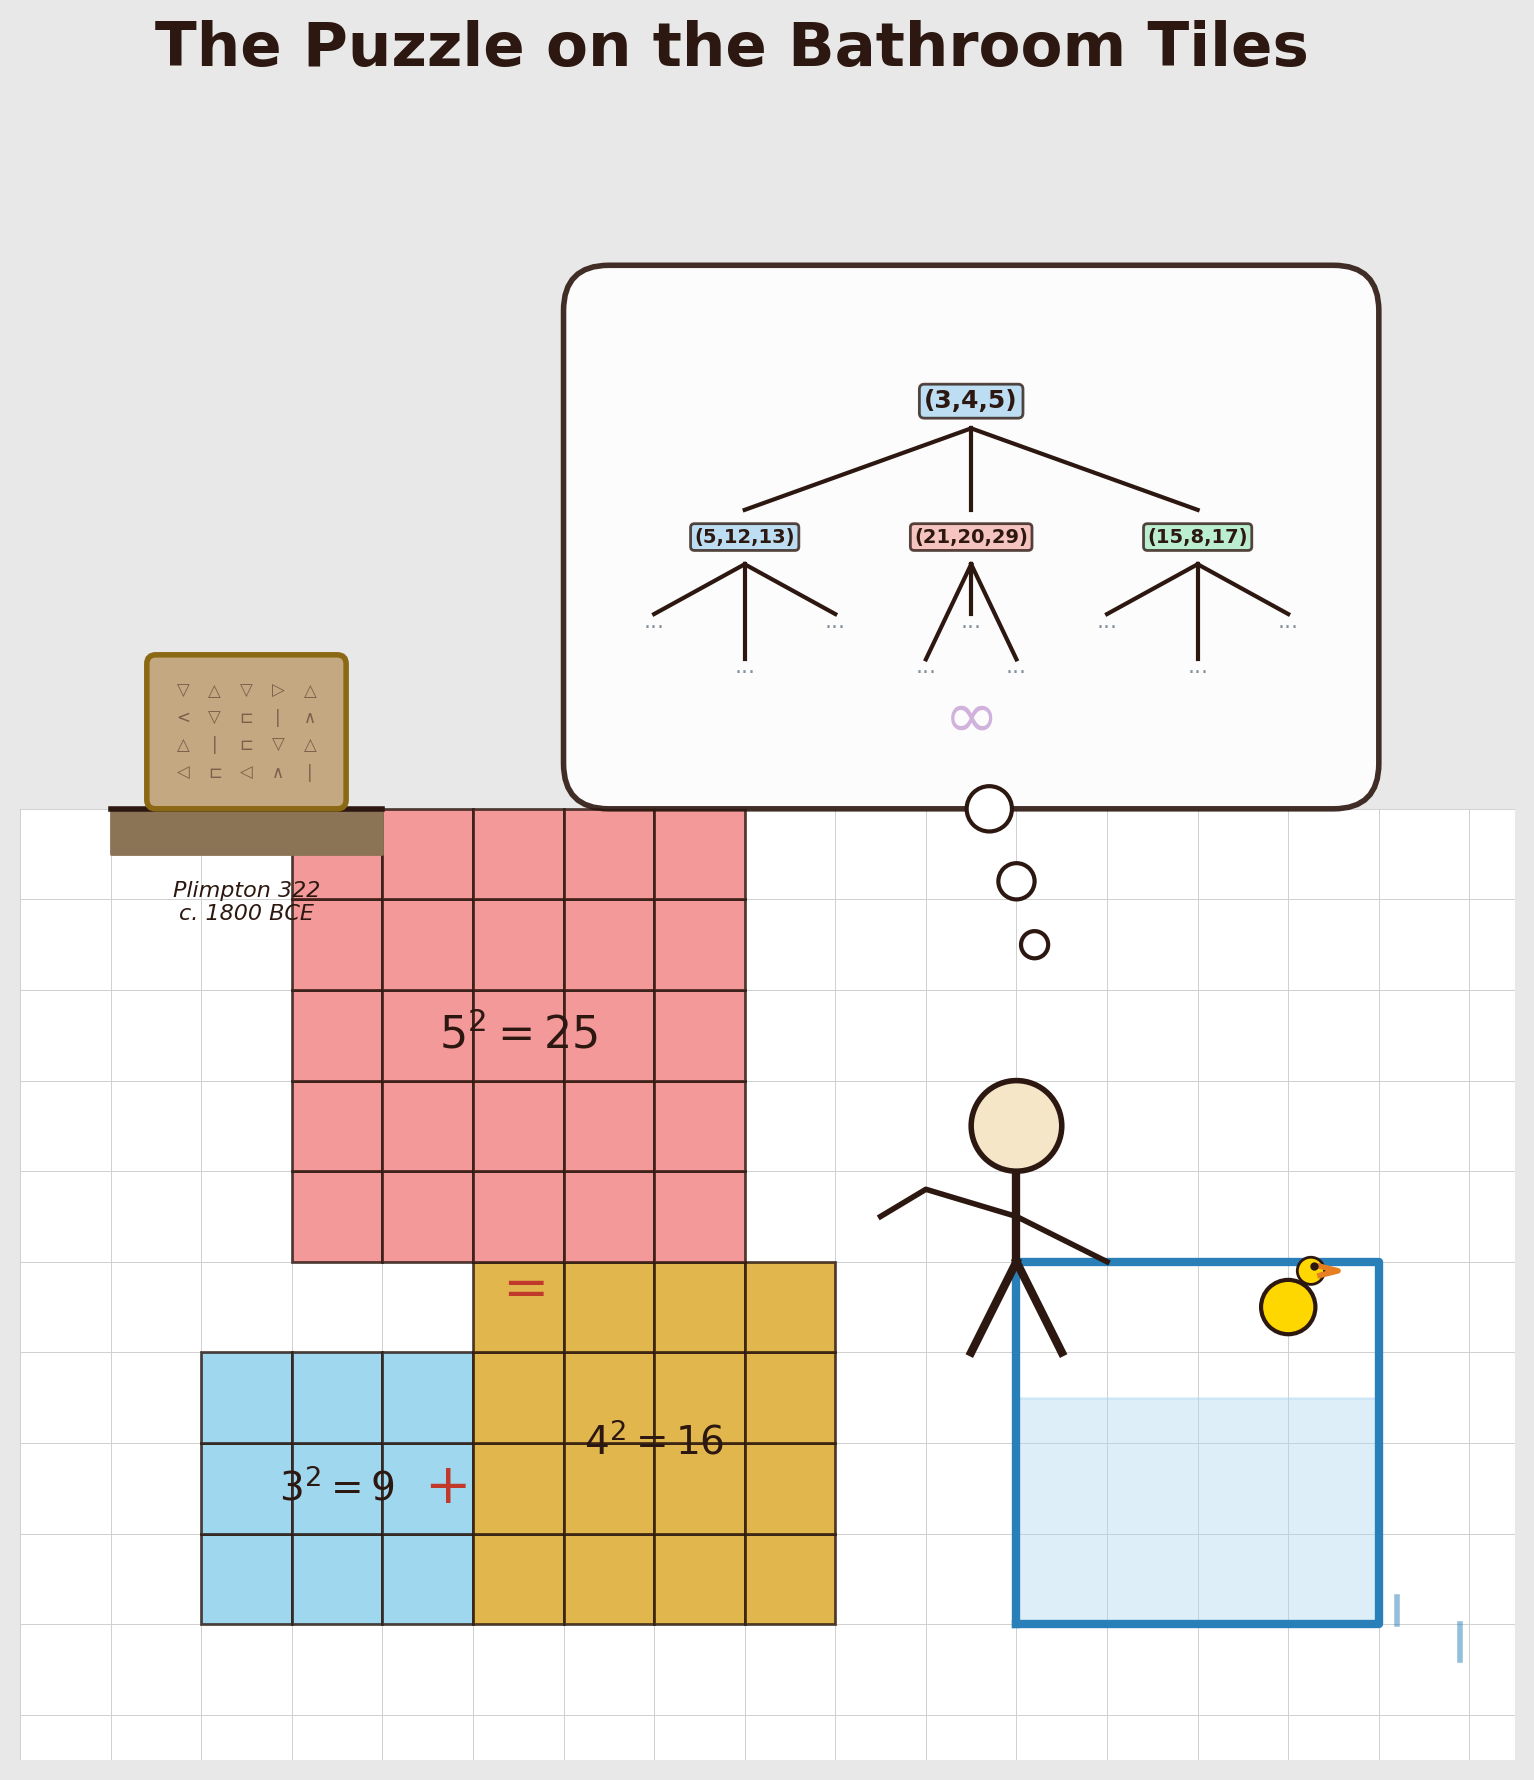
\includegraphics[width=0.82\textwidth,keepaspectratio]{images/introduction_fig03_bathroom_scene.png}
\caption{A whimsical, full-page scene depicting a person sitting on the edge of a bathtub, staring at a bathroom floor tiled with white unit squares.}
\end{figure}


What comes next will surprise you. Those sixteen triples are not scattered randomly across the number line like grains of sand on a beach. They are the first sixteen leaves of a single, infinite, perfectly ordered tree --- a tree whose branches are built from three matrices, whose geometry lives in hyperbolic space, and whose deepest symmetry is the symmetry of spacetime\index{spacetime} itself.

Turn the page, and let us begin to climb.

